%\chapter{Recuperación de información: getData} \label{append:getData}

\begin{center}
    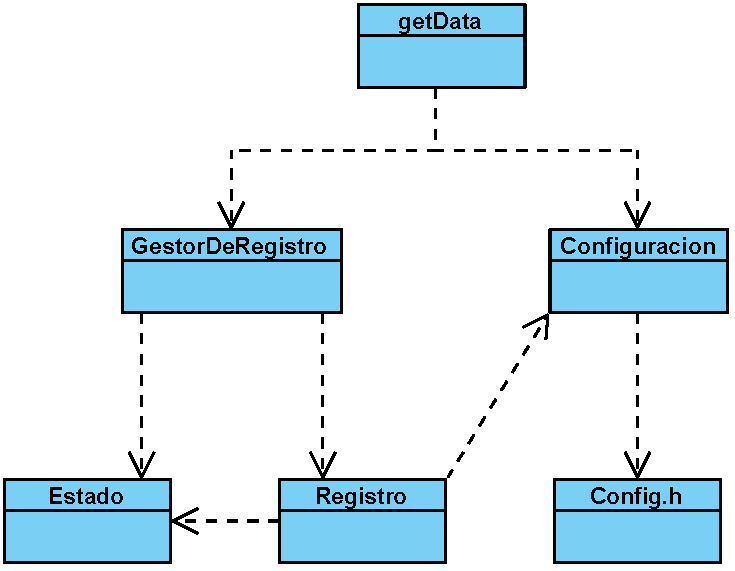
\includegraphics[width=0.9\textwidth]{figuras/lms11-getData.pdf}
    \captionof{figure}{Diagrama de clases del programa getData.}
    \label{fig:getData}
\end{center}

El programa \verb|getData| se encarga de recuperar los registros almacenados por el limitador pertenecientes a un intervalo de tiempo determinado, devolviéndolos en formato JSON. \verb|getData| recibe 4 parámetros y la sintáxis para invocarlo es la siguiente: \\

\begin{center}
    \verb|./getData $formato $fechaIni $fechaFin $intervalo|
\end{center}

donde:

\begin{itemize}
    \item Formato: \acrshort{XML} o \acrshort{JSON}
    \item Fecha de inicio: desde la fecha base del registro hasta la fecha actual.
    \item Fecha de fin: desde la fecha de inicio hasta la fecha actual.
    \item Intervalo de muestreo: intervalo de tiempo entre cada registro, en minutos.
\end{itemize}
La fechas van en el formato \verb|YYYY/MM/DD-hh:mm|, siguiendo el estándar \textbf{ISO 8601}.

Los listados \ref{lst:lm7-getData} y \ref{lst:lm9-getData} muestran los esquemas JSON devueltos por este programa en cada una de las versiones. \\
\begin{lstlisting}[
    language=json,
    label={lst:lm7-getData},
    caption={Esquema JSON devuelto por getData en las versión LM7.}
]
{
  "definitions": {
    "data": {
      "type": "object",
      "properties": {
        "registries": {
          "type": "array",
          "items": {
            "$ref": "#/definitions/Registry"
          }
        }
      }
    },
    "Registry": {
      "type": "object",
      "properties": {
        "time": {
          "type": "string"
        },
        "mic": {
          "type": "number"
        },
        "leftline": {
          "type": "number"
        },
        "rightline": {
          "type": "number"
        },
        "attenuation": {
          "type": "integer"
        },
        "maximum": {
          "type": "number"
        },
        "disconnectedMicrophone": {
          "type": "string",
          "format": "integer"
        }
      }
    }
  }
}
\end{lstlisting}

\vspace{1em}

\begin{lstlisting}[
    language=json,
    label={lst:lm9-getData},
    caption={Esquema JSON devuelto por getData en las versiones LM9 y LM11.}
]
{
  "definitions": {
    "data": {
      "type": "object",
      "properties": {
        "registries": {
          "type": "array",
          "items": {
            "$ref": "#/definitions/Registry"
          }
        }
      }
    },
    "Registry": {
      "type": "object",
      "properties": {
        "time": {
          "type": "string"
        },
        "mic": {
          "type": "number"
        },
        "leftline": {
          "type": "number"
        },
        "rightline": {
          "type": "number"
        },
        "attenuation": {
          "type": "integer"
        },
        "maximum": {
          "type": "number"
        },
        "disconnectedMicrophone": {
          "type": "string",
          "format": "integer"
        },
        "microphone": {
          "type": "array",
          "items": {
            "type": "number"
          }
        },
        "left": {
          "type": "array",
          "items": {
            "type": "number"
          }
        },
        "right": {
          "type": "array",
          "items": {
            "type": "number"
          }
        }
      }
    }
  }
}
\end{lstlisting}

%Esquemas generados a partir de muestras JSON del programa, mediante el uso de las herramientas \url{www.json-schema.org} y \url{www.jsonschemavalidator.net}.